\documentclass[conference]{IEEEtran}
\IEEEoverridecommandlockouts
% The preceding line is only needed to identify funding in the first footnote. If that is unneeded, please comment it out.
\usepackage{cite}
\usepackage{amsmath,amssymb,amsfonts}
\usepackage{algorithmic}
\usepackage{graphicx}
\usepackage{textcomp}
\usepackage{multirow}
\usepackage{xcolor}
\usepackage{xspace}
\def\BibTeX{{\rm B\kern-.05em{\sc i\kern-.025em b}\kern-.08em
    T\kern-.1667em\lower.7ex\hbox{E}\kern-.125emX}}
\begin{document}

\newcommand{\etal}{{\it et al.}\xspace}
\newcommand{\eg}{{\it e.g.}\xspace}

\title{Configurable Hardware Accelerator of Misuse-Resistant Authenticated Encryption for Tightly-Constrained Environments}
\author{\IEEEauthorblockN{Mustafa~Khairallah}
\IEEEauthorblockA{\textit{School of Physical and Mathematical Sciences} \\
\textit{Nanyang Technological University}\\
Singapore, Singapore \\
mustafa.khairallah@ntu.edu.sg
}
}

\maketitle

\begin{abstract}
  Nonce misuse is a frequently overlooked threat in tightly-constrained environments, either because of a gap of understanding between cryptographers and hardware designers, or because the solutions to such problem are presumed to be prohibitively expensive. The efforts to standardize a lightweight authenticated-encryption algorithm are coming to a close soon, yet only one candidate includes a nonce-misuse variant; Romulus-M, and its performance is almost not studied in practice. In this paper, study the performance of this algorithm in comparison to other AEAD schemes, specially its non-misuse-resistant variant; Romulus-N. We provide a family of configurable accelerators for both Romulus-N and Romulus-M, showing that the cost of adding Romulus-M with Romulus-N in the same implementations is very small in terms of area. We show that Romulus-M is less than 50\% slower than Romulus-N for short messages, and less 60\% slower for long messages, for low-area iterative configurations. We study the performance compared to other lightweight cryptography standardization candidates and other AEAD schemes. We also provide the first hardware implementations of Romulus compatible with both Tweakable Block Ciphers in the ISO/IEC NP 18033-7 standard proposal, with support for both Skinny and Deoxys-BC TBCs. The pre-synthesis configurations of our accelerator include choosing the TBC, the latency of the TBC, bus width and the number of plaintext and key shares (for masked implementations). During runtime, the user can select between Romulus-N and Romulus-M using input instructions. Finally, results are presented for both ASIC and FPGA, showing that Romulus-M is a competitive candidate in its own regard.
\end{abstract}

\begin{IEEEkeywords}
component, formatting, style, styling, insert
\end{IEEEkeywords}

\section{Introduction}


\section{Background}

\subsection{Nonces}

The security of SKE is dependent, by definition, on the secrecy of a shared secret key $K$ between communicating parties. In practice, however, the security of many SKE schemes, including most AEAD schemes, relies also on the properties of another parameter that is usually public, and is referred to as a Nonce $N$ or an Initial vector $IV$. This public parameter is usually assumed to be unique and cannot be repeated for two different messages (nonce-based AEAD) or uniformly random ($IV$-based AEAD).

Both of the aforementioned requirements are hard to enforce in practice. They rely on a threat model that assumes the user and implementer are both honest and understand the security requirements. To the contrary, it was shown that these assumptions may not hold even in widely-used commercial products, designed with the promise of hardware security. In February 2022, Shakevsky \etal showed an $IV$-reuse attack on the AES-GCM encryption algorithm on a range of flagship Android-powered Samsung smartphones~\cite{}.

Such attacks necessitate more careful handling of nonces. This can be done in one of two ways.

\begin{enumerate}

\item Ensure the implementations use nonces that satisfy the assumptions that the AEAD scheme is based on, \eg uniqueness. However, this approach is what is being assumed currently. This leads either complicated and costly implementations, or implementation mistakes that can leads to cryptographic breaks.

\item Rely on AEAD schemes that are more robust to nonce repetition or non-randomness. On the bright side, this issue have been studied by cryptographers, schemes such as SIV, AES-GCM-SIV, SCT, Deoxys-II and, more recently, Romulus-M.

\end{enumerate}

\subsection{Release of Unverified Plaintext}

Another challenge that faces efficient AEAD schemes is handling unverified ciphertexts. Several AEAD schemes need to decrypt the full ciphertext as part of the verification algorithm. However, standard definitions of AEAD do not take into account the security risks involved with releasing the unverified plaintext. This led Andreeva \etal~\cite{} proposed the Release of Unverified Plaintext security notion which takes this into account. This is useful for devices and implementations that do not have access to a large secure memory, where the unverified plaintext has to be stored in the main memory and/or transmitted to different destinations immediately.

Andreeva \etal also showed that it is possible to achieve such security notion in practice, using the SIV scheme. Recently, more RUP-secure schemes have been proposed. Iwata \etal~\cite{newresultsromulus} showed that Romulus-M achieves this security notion.

\begin{figure*}[!t]
  \centering
  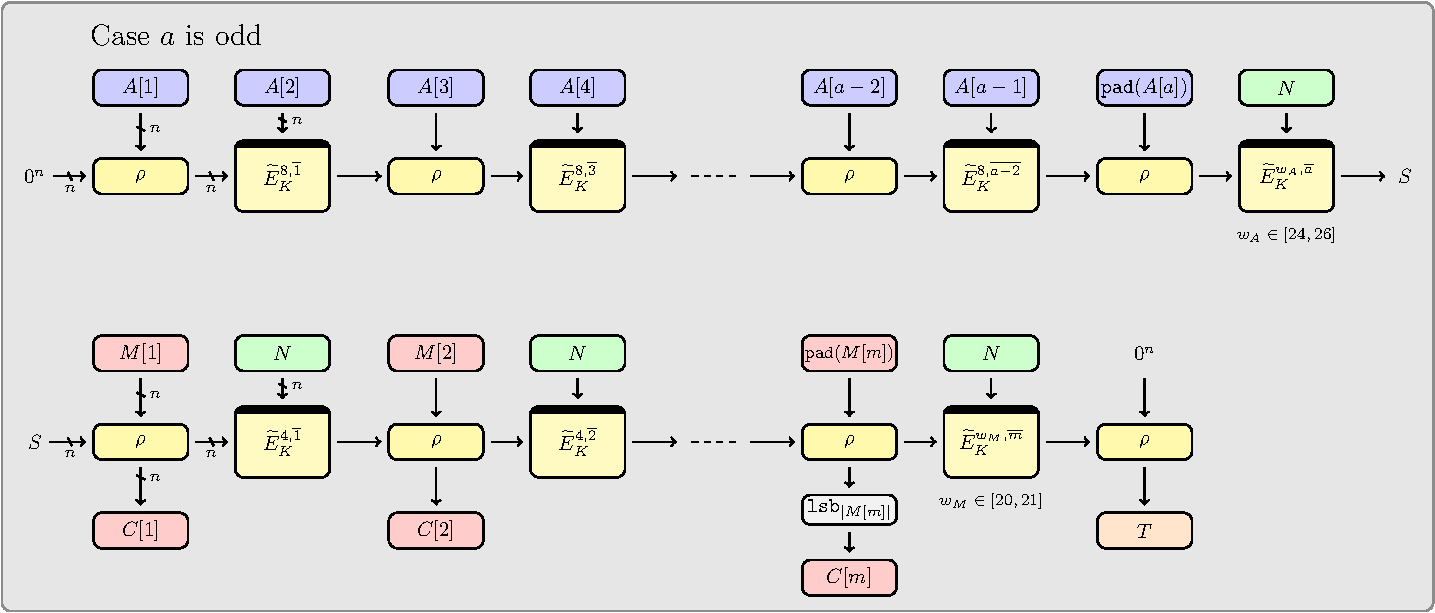
\includegraphics[width=\textwidth]{figures/mode_simplified.pdf}
  \caption{The Romulus-N AEAD scheme.}\label{fig:romulusn}
\end{figure*}

\subsection{Romulus}

Romulus~\cite{romulusspecs} is a finalist in the NIST lightweight cryptography competition. It is based on the Skinny TBC and incurs almost zero overhead in terms of storage compared to the underlying TBC. The schemes presented, however, are independent of the underlying TBC~\cite{romulusduel}. Romulus is a family of 4 SKE schemes:

\begin{enumerate}
\item {\it Romulus-N} is a nonce-respecting AEAD scheme, depicted in Figure~\ref{fig:romulusn}.
\item \item {\it Romulus-M} is a misuse-resistant AEAD scheme, depicted in Figure~\ref{fig:romulusm}.
\item {\it Romulus-H} is a hash function.
\item {\it Romulus-T} is a leakage-resilient AEAD scheme.
\end{enumerate}

Romulus-N is the main variant of the Romulus family, and almost all of the analysis and benchmarking have been done on this variant. However, Romulus-N fails under the security threats. Romulus-M, on the other hand, ensures security even in the presence of nonce-misuse and RUP. While Romulus-T offers security in the presence of side-channel leakage (under certain assumptions on the implementations), it does not offer privacy with nonce-misuse. Hence, we focus in this paper on Romulus-M and compare it to Romulus-N, showing that it can indeed be a more attractive option for sensitive lightweight applications and can have competitive performance compared to other lightweight schemes.

\begin{figure*}[!t]
  \centering
  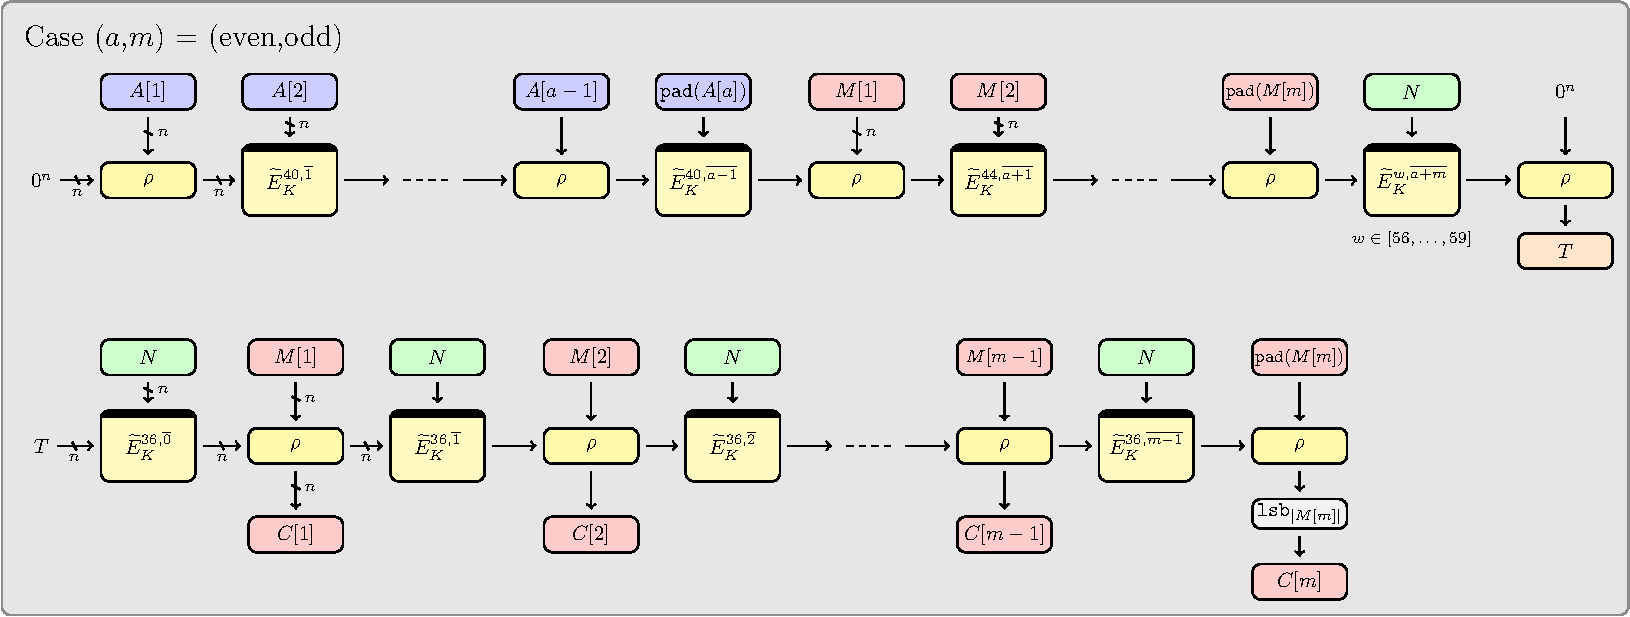
\includegraphics[width=\textwidth]{figures/modeM_simplified.pdf}
  \caption{The Romulus-M AEAD scheme.}\label{fig:romulusm}
\end{figure*}

\subsection{Tweakable Block Ciphers}

A TBC is a keyed function $\tilde{E}$ that takes three inputs: a secret key $K$, a public tweak $T$ and an $n$-bit message block $M$. For each selection of $(K,T)$, it behaves as a random permutation over the space of $n$-bit binary strings. A TBC is superior to a classical BC due to the extra public tweak $T$. TBCs have been formalized in~\cite{liskov} and have been a useful tool in the field of SKE encryption and design for years.Since the introduction of the $\Theta$CB-3~\cite{} and the design of the Deoxys-BC~\cite{}, more and more research have been performed in order to design practical, efficient and cheap TBCs and TBC-based schemes. Recently, two TBCs have been considered for the final stages of ISO standardization; Deoxys-BC~\cite{} and SKINNY~\cite{}. Deoxys-BC is the basis of Deoxys~\cite{}, the winned of the CAESAR competition for AEAD designs. SKINNY, on the other hand, is the basis for Romulus, a finalist in the NIST lightweight cryptography standardization project. 

\section{ISO/IEC NP 18033-7: Deoxys-BC and SKINNY}

The ISO/IEC NP 18033-7 is currently in the {\it ``under-review''} stage. It specifies the two TBCs: SKINNY and Deoxys-BC. In this section, we look at there combinational cost of there largest variants, with block size of 128 and tweakey size of 384. We assume they are used either as CPU co-processor or inside an iterative hardware accelerator that operates on the full 512-bit state in a single clock cycle. Hence, the smallest implementation is the round-based implementation; the combinational circuit performs 1 round per call/clock cycle. Deoxys-BC and SKINNY share similar design principles and they are both based on the tweakey framework. They are both based on the STK framework~\cite{} and Substitution-Permutation Networks (SPNs). Each round consists of 4 operations: SBoxLayer, AddRoundTweakey, ShiftRows, and MixColumn, with slightly different order. Deoxys-BC has an extra AddRoundTweakey operation in the final round. A common idea about lightweight ciphers is that they are targeted for constrained environments and are not suitable for high-speed applications. Our experiments on SKINNY and Deoxys-BC show that for most use-cases, this is not true. Deoxys-BC is only faster than SKINNY at very high frequencies, and this comes at a huge cost. In practice, the frequency will be decided by other parts of the system; {\it e.g.} CPU, Finite State Machine (FSM)...{\it etc.} 

We assume that all calls have the same number of rounds, such the combinational circuit of SKINNY can perform 1, 2, 4, 5, 8, 10, 20 or 40 rounds, while the circuit of Deoxys-BC can perform 1, 2, 4, 8, or 16 rounds. Since Deoxys-BC uses the AES round function, we considered two possible configurations for the SBox: Look-Up Table (LUT), which is more suitable for high-speed and FPGA implementations, as discussed in~\cite{}, and the Boyar-Peralta SBox circuit~\cite{}, which suitable for low-area ASIC implementations. Table~\cite{tab:comptbc} shows the synthesis results for these configurations on the TSMC 65nm standard cell library. While the speed of a hardware accelerator or an SoC is not determined just by the cryptographic combinational circuit, this section can be viewed as investigating the limits of these TBCs. For example, Table~\cite{tab:comptbc} shows that the circuit cannot be computed on the considered technology in with less than 17.4ns, while Deoxys-BC cannot computed in less than 12.91ns. When we add a 0.5ns safety slack per call, these numbers grow to 19.97ns and 13.4, respectively. However, when we also compare the area, we see that the faster implementation of Deoxys-BC comes at a huge area cost, where the fastest implementation of SKINNY costs 2228.75 and 52892.5, respectively, while for Deoxys-BC, the best latency is achieved at 174169.24 GE. SKINNY also has the potential to be 7 times more efficient than Deoxys-BC at high frequencies, and 2.3 times more efficient at 24 MHz. At low frequencies, the efficiency of both TBCs becomes almost constant, in which case they both offer an interesting straight-forward trade-off between speed and area. Note that these values are only for the combinational part of the cipher, and the efficiencies will drop when the storage is added. However, we exclude the storage from this section as the storage should be part of the higher-level system. In the next section, we will revisit how SKINNY and Deoxys-BC can be used inside existing systems without requiring any extra storage.

\begin{table*}[!thb]
\centering
\caption{Comparison of the logic circuit of Skinny and Deoxys-BC for different value of latency. Synthesis results are using TSMC 65nm.}\label{tab:comptbc}
\begin{tabular}{c|c|c|c|c|c|c|c|c}\hline
  \multirow{2}{*}{\textbf{TBC}} & \multirow{2}{*}{\textbf{\# of Rnds}} & \multirow{2}{*}{\textbf{\# of Cycles}} & \textbf{Area} & \textbf{Critical Path} & \textbf{Min. Latency} & \textbf{Safe Latency} & \textbf{$\frac{128000}{L\times A}$}  & \multirow{2}{*}{\textbf{$\frac{128000}{L\times A}$ at 24MHz}} \\
  & & & \textbf{(GE)} & \textbf{(ns)} & \textbf{(ns)} & \textbf{(ns)} & \textbf{at min. latency.} & \\ \hline \hline
  \multirow{8}{*}{Skinny} &
    1	& 40 & 1107 & 0.44	& 17.6	& 37.6 & 6.57 & 0.07 \\
  & 2	& 20 & 2228.75 & 0.87	& 17.4	& 27.4 & 3.3 & 0.07 \\
  & 4	& 10 & 4790.5 & 1.94	& 19.4	& 24.4 & 1.37 & 0.06 \\ 
  & 5	&  8 & 6029.5 & 2.56	& 20.48	& 24.48 & 1.03 & 0.06 \\
  & 8	&  5 & 10117 & 3.86	& 19.3	& 21.8 & 0.66 & 0.06 \\
  & 10 & 4 & 12776.75 & 4.94	& 19.76	& 21.76 & 0.51 & 0.06 \\
  & 20 & 2 & 26554.68 & 9.78	& 19.56	& 20.56 & 0.25 & 0.06 \\
  & 40 & 1 & 52892.5 & 19.47 & 19.47 & 19.97 & 0.12 & 0.06 \\
    \hline
    \multirow{5}{*}{Deoxys-BC LUT} &
    1 & 16 & 9825.25& 0.88 & 14.08 & 22.08 & 0.93 & 0.02 \\
    & 2 & 8 & 20998& 1.7 & 13.6 & 17.6 & 0.45 & 0.02 \\
    & 4 & 4 & 43588.5& 3.4 & 13.6 & 15.6 & 0.22 & 0.02 \\
    & 8 & 2 & 86156.25& 6.65 & 13.3 & 14.3 & 0.11 & 0.02 \\
    & 16 & 1 & 174169.24& 12.91 & 12.91 & 13.4 & 0.06 & 0.02 \\
    \hline
    \multirow{5}{*}{Deoxys-BC BP} &
    1 & 16 & 7347.25& 1.26 & 20.16 & 28.16 & 0.86 & 0.03 \\
    & 2 & 8 & 19346 & 2.39 & 19.12 & 23.12 & 0.35 & 0.02 \\
    & 4 & 4 & 43634 & 4.43 & 17.72 & 19.72 & 0.17 & 0.02 \\
    & 8 & 2 & 91086.11& 8.78 & 17.56 & 18.56 & 0.08 & 0.02 \\
    & 16 & 1 & 181776 &  16.71 &  16.71 &  17.21 &  0.04 & 0.02 \\ \hline
\end{tabular}
\end{table*}



\section{Romulus-N/M Hardware Accelerator}

\begin{figure*}[!htb]
  \centering
  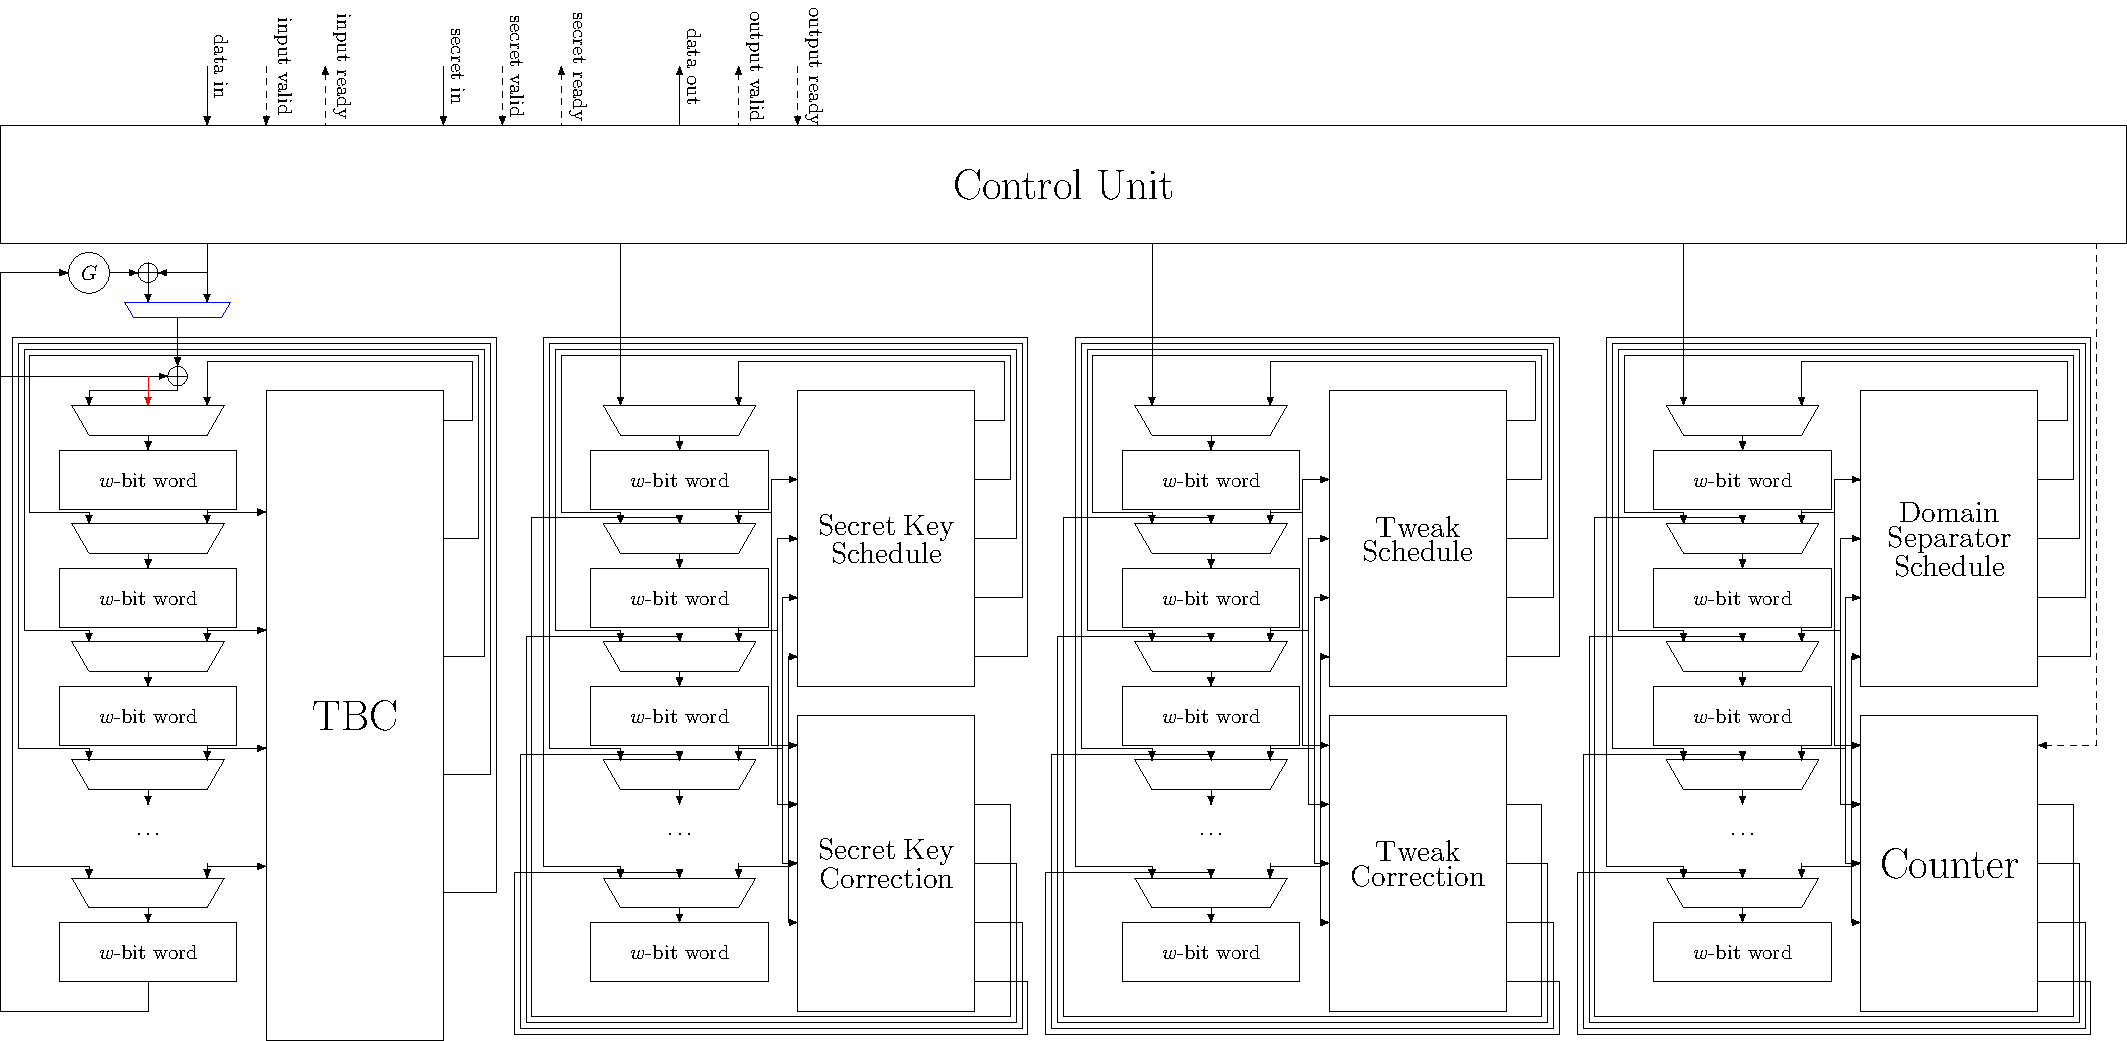
\includegraphics[width=\textwidth]{arch_diagram.pdf}
  \caption{The architecture of the proposed hardware accelerator. Solid arrow are $w$-bit wide, where $w$ is the configurable bus width. The dotted arrows are control signals. Some of the control signals are omitted from the diagram for simplicity including multiplexers' selectors, registers enables and resets. The red arrow is only needed for Romulus-M and can be removed if Romulus-M support is not required. The blue multiplexer is used to switch between encryption and decryption.}\label{fig:arch}
\end{figure*}

\begin{table}[!thb]
  \centering
  \caption{Latency of Romulus-N and Romulus-M for different latencies of the TBC.}\label{tab:instlatency}
  \begin{tabular}{c|c|c|c|c|c|c|c}\hline
  \textbf{Mode} & \textbf{$a$} & \textbf{$m$} & 1 & 2 & 4 & 10 & 40 \\\hline \hline
  \multirow{10}{*}{N} & 0 & 0 & 101 & 61 & 41 & 29 & 23 \\
  &  0 & 16 & 101 & 61 & 41 & 29 & 23 \\
  & 16 &  0 & 101 & 61 & 41 & 29 & 23 \\
  & 16 & 16 & 101 & 61 & 41 & 29 & 23 \\
  &  0 & 64 & 237 & 137 & 87 & 57 & 42 \\
  & 64 &  0 & 197 & 117 & 77 & 53 & 41 \\ 
  & 64 & 64 & 333 & 193 & 123 & 81 & 60 \\
  & 0 & 1152 & 3225	& 1765	& 1035	& 597	& 378 \\
  & 1152 & 0 & 1825	& 1065 &	685	& 457	& 343 \\
  & 1152 & 1152 & 4949 & 2769 & 1679	& 1025 & 698 \\ \hline

  \multirow{10}{*}{M} & 0 & 0 & 101	& 61	& 41	& 29	& 23 \\
  &  0 & 16 & 146	& 86 &	56	& 38	& 29 \\
  & 16 &  0 & 101	& 61	& 41	& 29	& 23 \\
  & 16 & 16 & 146	& 86 & 56 & 38	& 29 \\
  &  0 & 64 & 338	&198	&128	&86	&65 \\
  & 64 &  0 & 157	& 97	&67	&49	&40  \\ 
  & 64 & 64 & 434	&254	&164	&110	&83 \\
  & 0 & 1152 & 4954	&2774	&1684	&1030	&703 \\
  & 1152 & 0 & 1785	&1045	&675	&453	&342 \\
  & 1152 & 1152 & 6678	&3778	&2328	&1458	&1023 \\ \hline

  & & & 1.00	& 1.00	& 1.00	& 1.00	& 1.00 \\
  & & & 1.45	& 1.41	& 1.37	& 1.31	& 1.26 \\
  & & & 1.00	& 1.00	& 1.00	& 1.00	& 1.00 \\
  & & & 1.45	& 1.41	& 1.37	& 1.31	& 1.26 \\
  Latency& & & 1.43	& 1.45	& 1.47	& 1.51	& 1.55 \\
  Overhead& & & 0.79	& 0.83	& 0.87	& 0.92	& 0.98 \\
  & & & 1.30	& 1.32	& 1.33	& 1.36	& 1.38 \\
  & & & 1.57	& 1.57	& 1.63  & 1.72	& 1.86 \\
  & & & 0.99	& 0.98	& 0.98	& 0.99	& 1.00 \\
  & & & 1.35	& 1.36	& 1.39	& 1.42	& 1.47 \\ \hline
  \end{tabular}
\end{table}

\begin{table*}
  \centering
  \caption{Our hardware accelerator using SKINNY on TSMC 65nm.}\label{tab:acc65nm}
  \begin{tabular}{c|c|c|c|c|c|c|c|c|c|c}\hline
    \multicolumn{2}{c|}{}&\multicolumn{4}{c|}{\textbf{24MHz}}&\multicolumn{4}{c}{\textbf{Max. Frequency}} \\ \hline
    \textbf{TBC} & \textbf{Area} & \textbf{CP} & \textbf{Power} & \textbf{Energy} & \textbf{Energy} & \multirow{2}{*}{\textbf{$\times$}} & \textbf{Power} & \textbf{Energy} & \textbf{Energy} & \multirow{2}{*}{\textbf{$\times$}} \\ 
    \textbf{Rounds} & \textbf{(GE)} & \textbf{(ns)} & \textbf{(mW)} & \textbf{(pJ/bit)} &  \textbf{(pJ/bit)} &  & \textbf{(mW)} & \textbf{(pJ/bit)} &  \textbf{(pJ/bit)}  & \\
    & & & & \textbf{N} & \textbf{M} & & & \textbf{N} & \textbf{M} & \\ \hline \hline
    1  & 7348.61   & 1.11	  & 0.221   & 2.47	& 3.33 & 1.35 & 0.74 & 0.30 & 0.40 & 1.35 \\ 
    2	 & 7865.28	 & 1.16		& 0.239		& 1.49	& 2.04 & 1.36 & 0.74 & 0.17 & 0.23 & 1.36 \\ 
    4	 & 10124.24	 & 1.9		& 0.318		& 1.21	& 1.67 & 1.37 & 0.70 & 0.13 & 0.18 & 1.39 \\ 
    10 & 17767.99	 & 5.03		& 0.59		& 1.36	& 1.94 & 1.42 & 0.73 & 0.21 & 0.30 & 1.42 \\ 
    40 & 55098.25	 & 19.25	& 1.94		& 3.06	& 4.47 & 1.47 & 1.96 & 1.48 & 2.17 & 1.47 \\ \hline 
  \end{tabular}
\end{table*}

\begin{table*}
  \centering
  \caption{Our hardware accelerator using Deoxys-BC (with Boyar-Peralta's SBox) on TSMC 65nm.}\label{tab:acc65nm}
  \begin{tabular}{c|c|c|c|c|c|c|c|c|c|c}\hline
    \multicolumn{2}{c|}{}&\multicolumn{4}{c|}{\textbf{24MHz}}&\multicolumn{4}{c}{\textbf{Max. Frequency}} \\ \hline
    \textbf{TBC} & \textbf{Area} & \textbf{CP} & \textbf{Power} & \textbf{Energy} & \textbf{Energy} & \multirow{2}{*}{\textbf{$\times$}} & \textbf{Power} & \textbf{Energy} & \textbf{Energy} & \multirow{2}{*}{\textbf{$\times$}} \\ 
    \textbf{Rounds} & \textbf{(GE)} & \textbf{(ns)} & \textbf{(mW)} & \textbf{(pJ/bit)} &  \textbf{(pJ/bit)} &  & \textbf{(mW)} & \textbf{(pJ/bit)} &  \textbf{(pJ/bit)}  & \\
    & & & & \textbf{N} & \textbf{M} & & & \textbf{N} & \textbf{M} & \\ \hline \hline
    1  & 18230.04  & 1.91	  & 0.431   & 2.47	& 3.33 & 1.35 & 0.74 & 0.30 & 0.40 & 1.35 \\ 
    2	 & 7865.28	 & 1.16		& 0.239		& 1.49	& 2.04 & 1.36 & 0.74 & 0.17 & 0.23 & 1.36 \\ 
    4	 & 10124.24	 & 1.9		& 0.318		& 1.21	& 1.67 & 1.37 & 0.70 & 0.13 & 0.18 & 1.39 \\ \hline
  \end{tabular}
\end{table*}

\section{Comparison with Lightweight AEAD Accelerators}


\begin{figure}[!h]
  \centering
  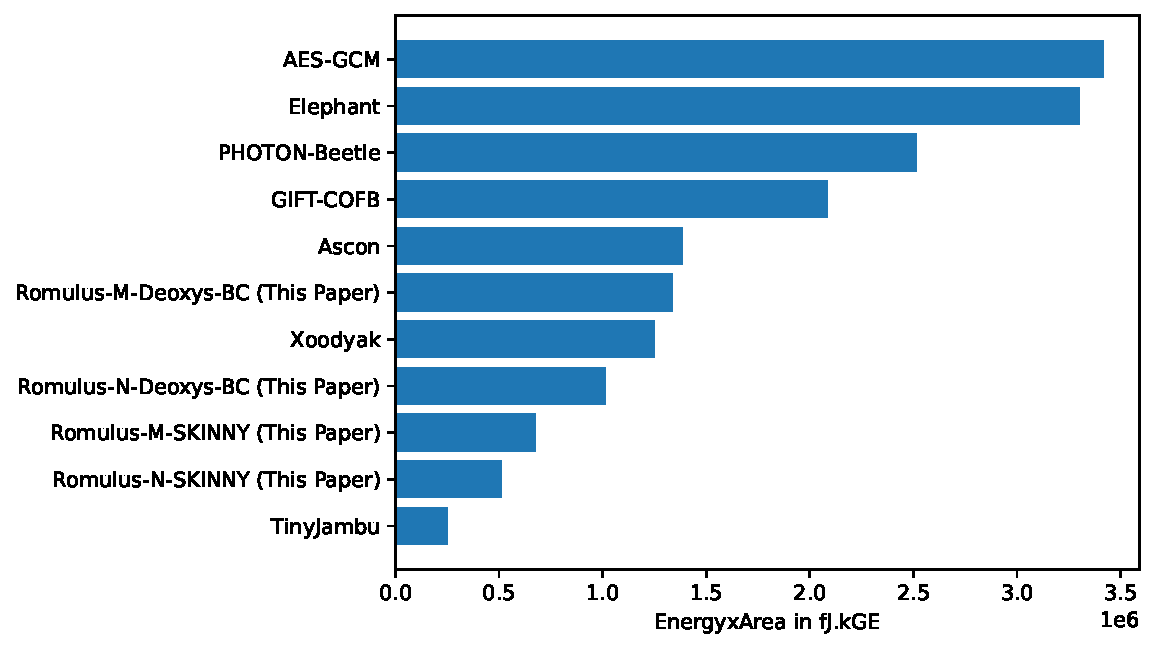
\includegraphics[width=0.49\textwidth]{figures/withM_energy_area64_bar_65.pdf}
  \caption{Energy$\times$Area product for 64 AD and message blocks for various AEAD schemes.}\label{fig:energy_area_64}
\end{figure}

\begin{figure}[!h]
  \centering
  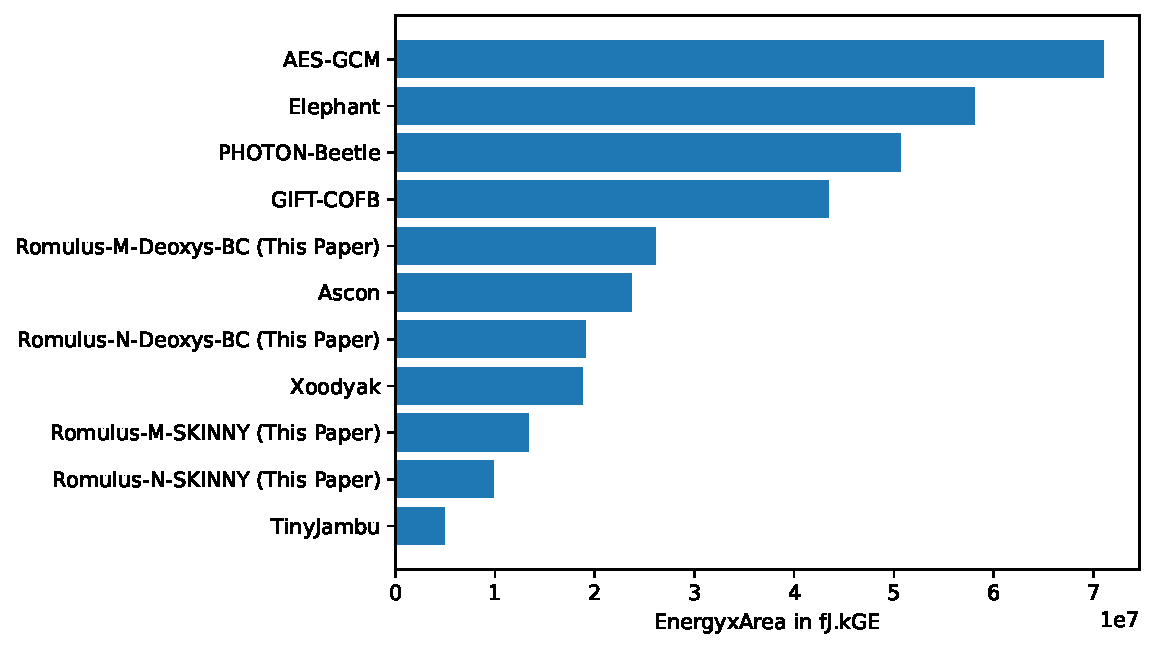
\includegraphics[width=0.49\textwidth]{figures/withM_energy_area1536_bar_65.pdf}
  \caption{Energy$\times$Area product for 1536 AD and message blocks for various AEAD schemes.}\label{fig:energy_area_1536}
\end{figure}

\begin{figure}[!h]
  \centering
  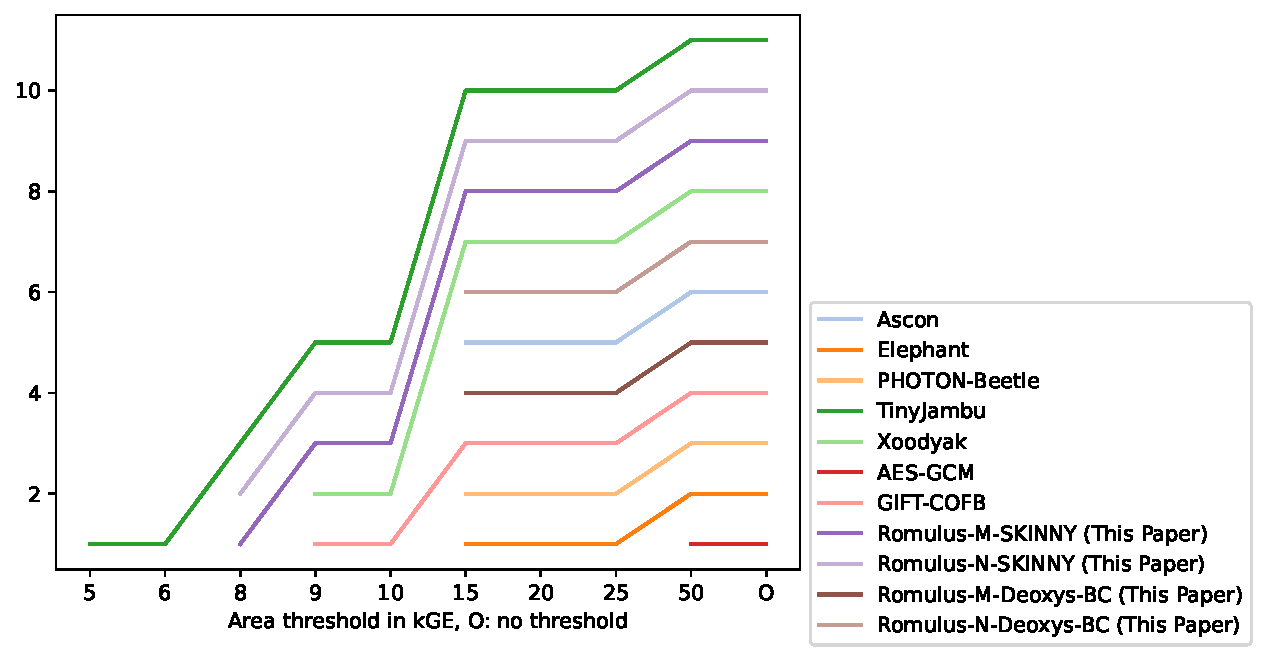
\includegraphics[width=0.49\textwidth]{figures/withM_energy_area1536_rank_65.pdf}
  \caption{Energy ranking vs Area for 1536 AD and message blocks for various AEAD schemes.}\label{fig:thoughput_1536}
\end{figure}

\begin{figure}[!h]
  \centering
  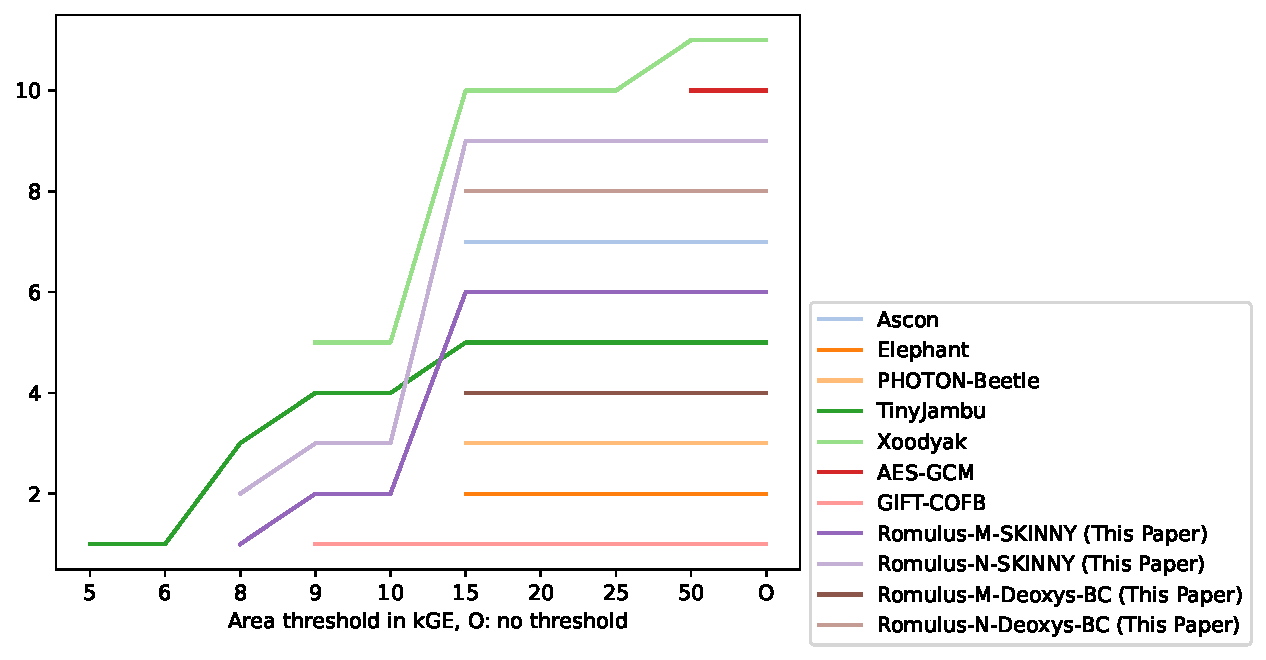
\includegraphics[width=0.49\textwidth]{figures/withM_throughput1536_rank_65.pdf}
  \caption{Through ranking vs. Area for 1536 AD and message blocks for various AEAD schemes.}\label{fig:thoughput_1536}
\end{figure}







\end{document}
